\documentclass[12pt,a4paper]{abntex2}

% Pacotes essenciais
\usepackage[utf8]{inputenc}
\usepackage[T1]{fontenc}
\usepackage{lmodern}
\renewcommand{\familydefault}{\sfdefault}
\usepackage[brazil]{babel}
\usepackage{graphicx}
\usepackage{indentfirst}
\usepackage{setspace}
\usepackage{geometry}
\usepackage{listings}
\usepackage{booktabs}
\usepackage{longtable}
\usepackage{graphicx}
\usepackage{amssymb}
\usepackage{float}
\geometry{a4paper,left=3cm,right=2cm,top=3cm,bottom=2cm}
\renewcommand{\thesection}{\arabic{section}}
\renewcommand{\thesubsection}{\thesection.\arabic{subsection}}
\renewcommand{\thesubsubsection}{\thesubsection.\arabic{subsubsection}}
\OnehalfSpacing
% =========================
% Configuração de listagens (ASCII / Saídas do Java)
% =========================
\lstdefinestyle{console}{
  basicstyle=\ttfamily\small,
  columns=fullflexible,
  frame=single,
  breaklines=true,
  keepspaces=true,
  tabsize=2
}

\begin{document}

% CAPA
\title{Relatório Técnico -- Comparativo de Funções Hash em Java}
\author{Fernando Alonso Piroga da Silva \\ Jafte Carneiro Fagundes da Silva \\ Renato Pestana Gouveia}
\date{\textbf{Pontifícia Universidade Católica do Paraná} \\ Resolução de Problemas Estruturados em Computação \\ Prof.ª Marina de Lara}
\maketitle

\tableofcontents
\newpage

% INTRODUÇÃO
\section{Introdução}
Este relatório apresenta o desenvolvimento e a análise comparativa de duas implementações de Tabelas Hash em Java, desenvolvidas manualmente, sem o uso de coleções prontas da linguagem. O objetivo do trabalho é avaliar a eficiência de diferentes funções de dispersão (hash functions) quanto à distribuição de chaves, número de colisões, tempo de execução e comportamento de redimensionamento.

O trabalho contempla: (i) implementação base abstrata; (ii) duas implementações concretas que diferem apenas na função hash; (iii) coleta de métricas; (iv) relatório comparativo. Os resultados numéricos e gráficos ASCII apresentados nas seções seguintes serão preenchidos com a saída do programa Java.


A Tabela Hash é uma estrutura de dados fundamental em Computação, permitindo operações de inserção e busca em tempo médio constante. No entanto, a eficiência depende fortemente da função hash utilizada e do tratamento de colisões.

Neste trabalho, as funções analisadas foram:

\begin{itemize}
  \item \textbf{Polynomial Rolling Hash}
  \item \textbf{DJB2}
\end{itemize}

Ambas as funções foram testadas sobre um conjunto de 5001 nomes provenientes do arquivo \texttt{female\_names.txt}, com capacidade inicial de 32 posições e fator de carga de 0,75.

\newpage

% DESENVOLVIMENTO
\section{Metodologia de Implementação}

\subsection{Arquitetura do Sistema}
A solução foi estruturada com ênfase em encapsulamento, abstração, herança e polimorfismo. A classe abstrata \texttt{TabelaHash} define a interface e a lógica comum, enquanto as subclasses implementam a função hash específica. O tratamento de colisões é feito via \textit{chaining} com \texttt{ListaEncadeada} e nós (\texttt{Node}) implementados manualmente.

\subsection{Diagrama de Classes}

\begin{figure}[h]
    \centering
    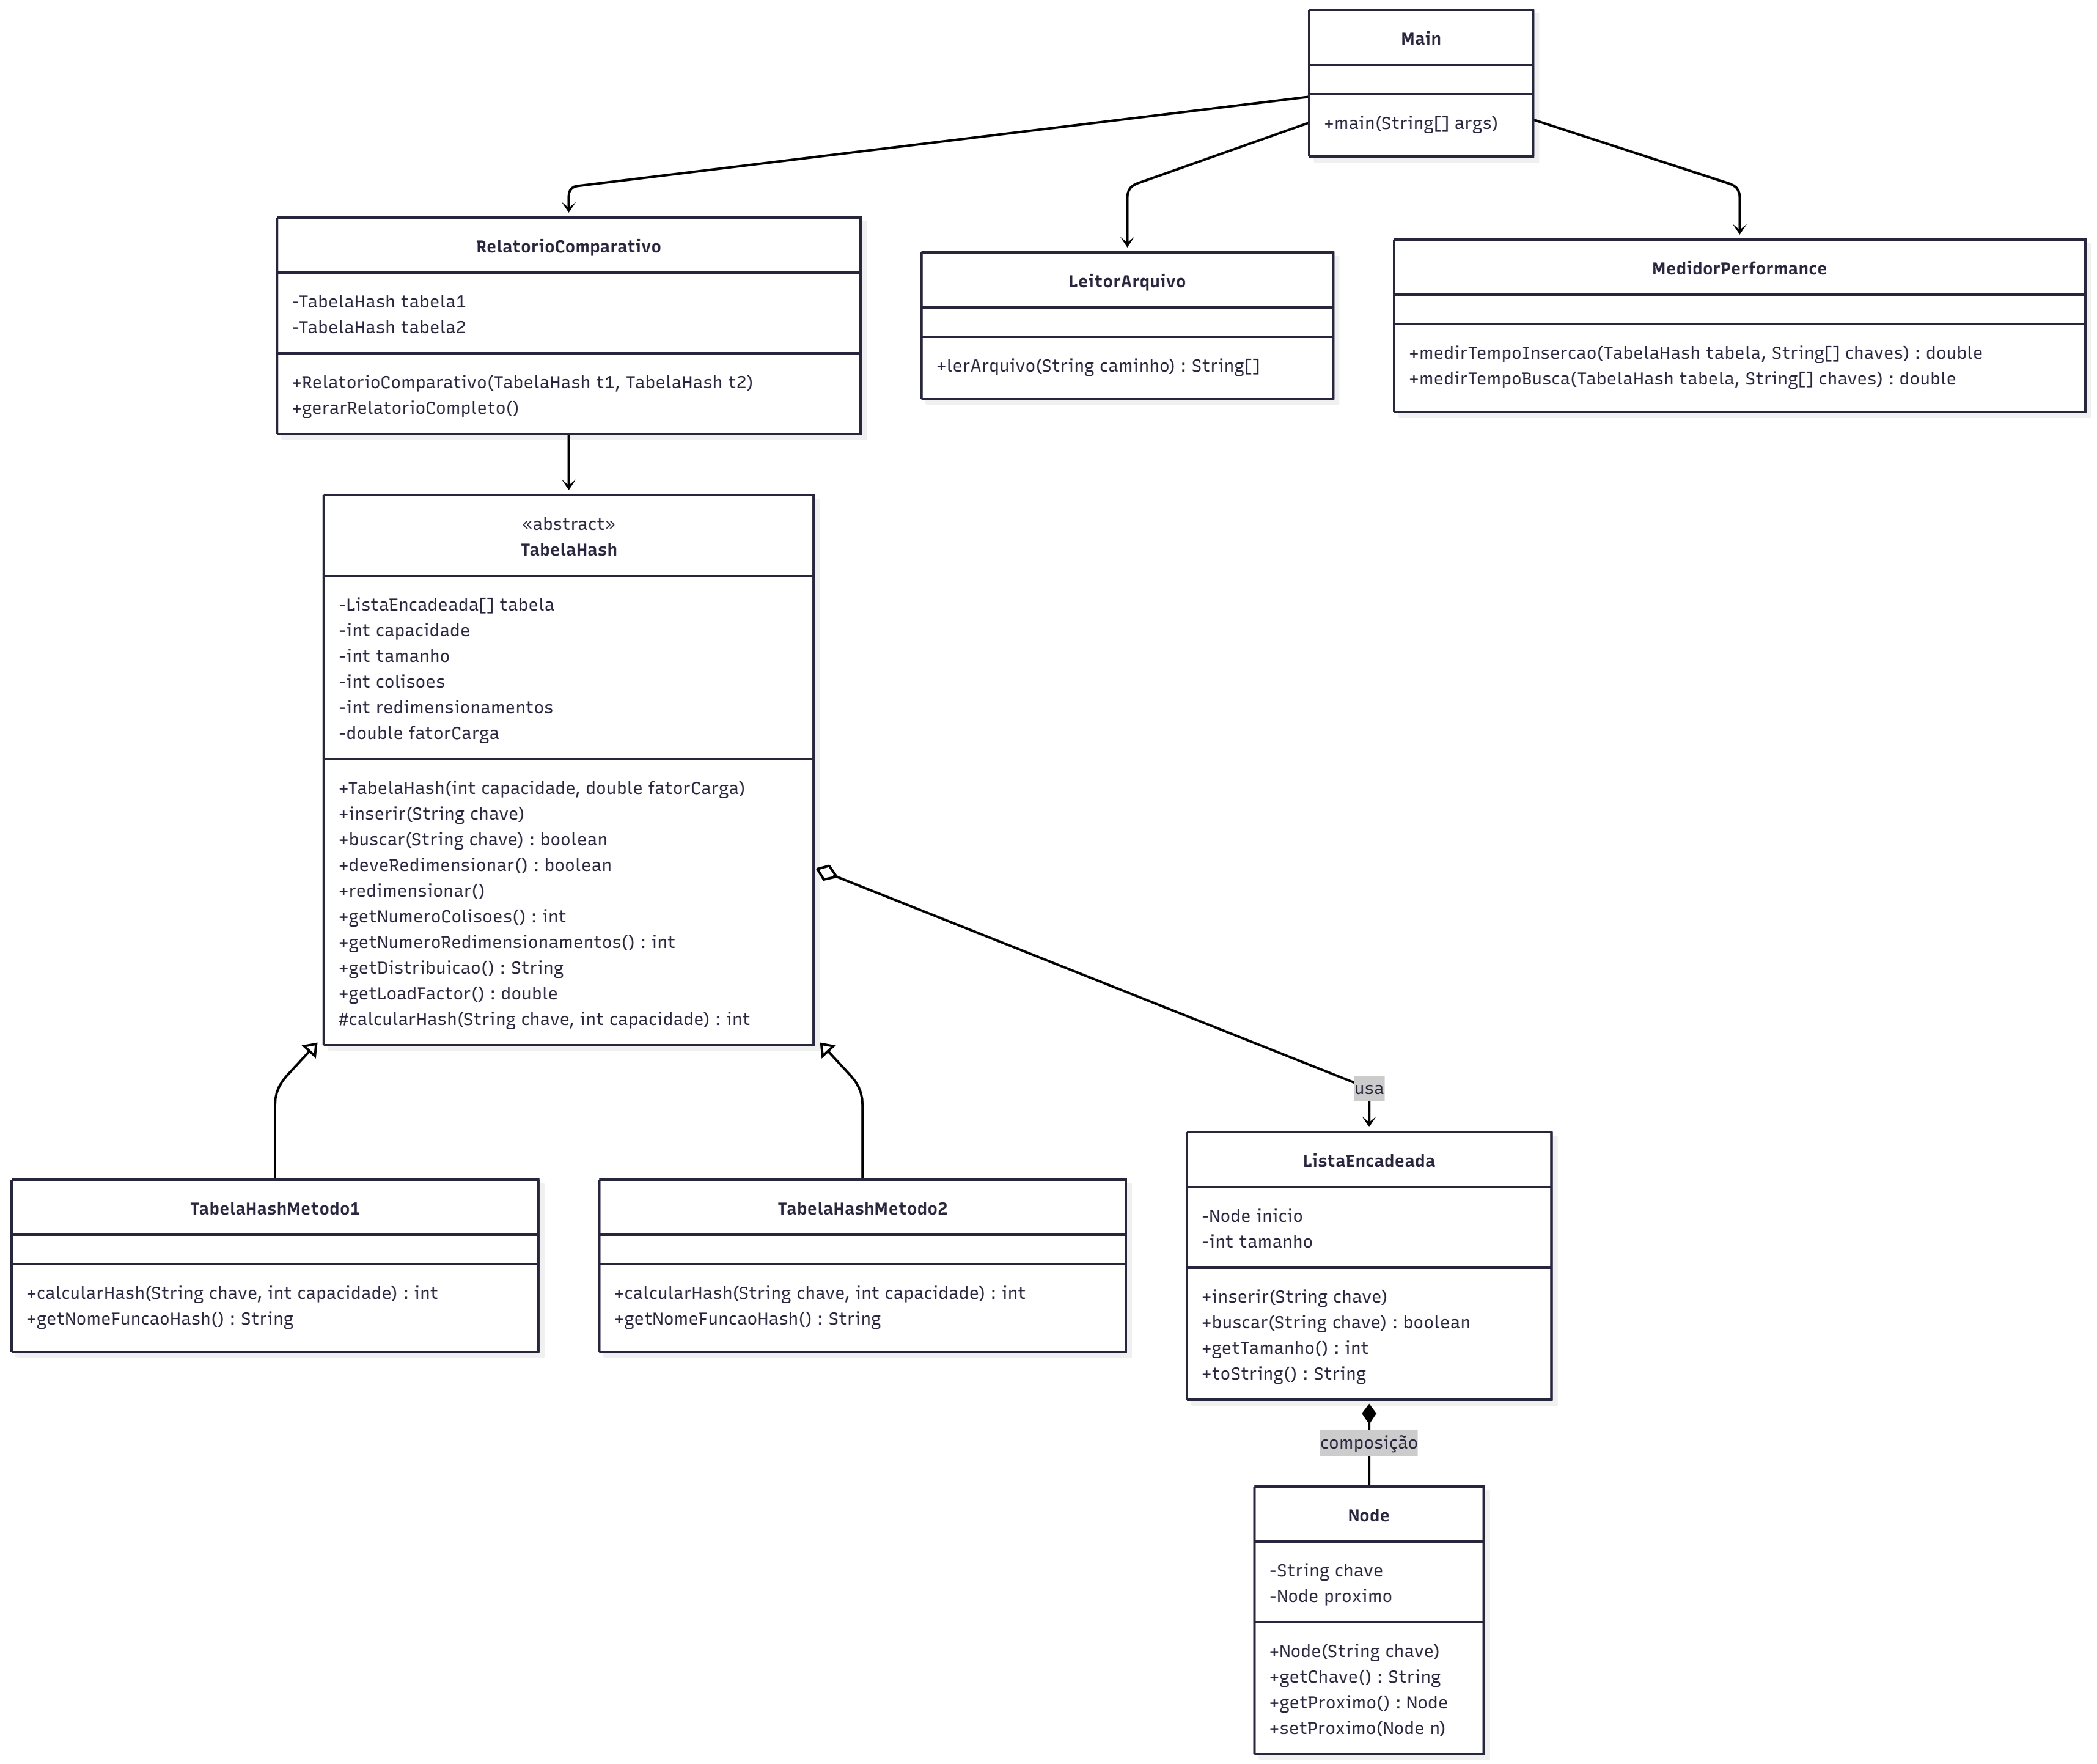
\includegraphics[width=1\textwidth]{DiagramClasses.png}
    \caption{Diagrama com a implementação das classes}
    \label{fig:minha_imagem}
\end{figure}


O projeto foi estruturado de forma orientada a objetos, com uma classe abstrata \texttt{TabelaHash} que define a estrutura base e o comportamento comum das tabelas. As classes concretas \texttt{TabelaHashMetodo1} e \texttt{TabelaHashMetodo2} sobrescrevem apenas o método de cálculo hash, garantindo baixo acoplamento e alto reuso de código.

\subsection{Tratamento de Colisões}
As colisões foram tratadas por \textbf{encadeamento} (\textit{chaining}), utilizando uma lista encadeada simples implementada manualmente (classes \texttt{ListaEncadeada} e \texttt{Node}). Cada posição da tabela mantém uma lista de elementos que compartilham o mesmo índice hash.

\subsection{Redimensionamento e Rehashing}
Quando o fator de carga atinge o limite de 0,75, a tabela dobra de tamanho e todos os elementos são \textit{re-hashados}  para a nova capacidade. Esse processo é contabilizado na métrica de redimensionamentos.

\subsection{Funções Hash Utilizadas}

\subsubsection{Função Hash 1 -- Polynomial Rolling Hash}
O \textit{Polynomial Rolling Hash} é uma função de dispersão amplamente utilizada em algoritmos de correspondência de padrões, como o Rabin-Karp.
Sua principal característica é representar a chave (string) como um polinômio, onde cada caractere contribui com um termo ponderado por uma base \(p\).
A soma é calculada sob um módulo grande \(M\), garantindo que o valor não ultrapasse os limites numéricos e reduzindo colisões.

Matematicamente, a função é definida como:

\[
h(s) = \left( \sum_{i=0}^{n-1} s_i \cdot p^i \right) \bmod M
\]

onde:
\begin{itemize}
  \item \(s_i\) é o valor ASCII do caractere \(i\)-ésimo da string;
  \item \(p\) é uma constante base (neste trabalho, \(p = 31\));
  \item \(M\) é um número primo grande (\(M = 10^9 + 9\)).
\end{itemize}

Após o cálculo, o valor absoluto é tomado e reduzido pelo operador módulo da capacidade da tabela, obtendo um índice entre \(0\) e \texttt{capacidade - 1}.

\subsubsubsection{Assinatura e Implementação (Java)}
\begin{lstlisting}[style=console]
@Override
protected int calcularHash(String chave, int capacidade) {
    long hash = 0;
    long p = 31;
    long m = 1000000009L;
    long power = 1;

    for (int i = 0; i < chave.length(); i++) {
        char c = chave.charAt(i);
        hash = (hash + (c - 'a' + 1) * power) % m;
        power = (power * p) % m;
    }

    return (int) (Math.abs(hash) % capacidade);
}
\end{lstlisting}


\subsubsection{Função Hash 2 -- DJB2}
A função \textit{DJB2} foi criada por Daniel J. Bernstein e é uma das mais conhecidas por combinar boa dispersão, simplicidade e desempenho.
Ela utiliza um processo iterativo de deslocamento e soma que distribui os bits da chave de forma eficiente.

O algoritmo começa com uma constante inicial (\(h_0 = 5381\)) e, para cada caractere \(c_i\) da string, realiza a atualização:

\[
h_i = \left( (h_{i-1} \ll 5) + h_{i-1} + c_i \right)
\]

ou, equivalentemente, \( h_i = 33 \cdot h_{i-1} + c_i \).
Ao final, o resultado é ajustado para um número positivo e mapeado para o intervalo da capacidade da tabela.

\subsubsubsection{Assinatura e Implementação (Java)}
\begin{lstlisting}[style=console]
@Override
protected int calcularHash(String chave, int capacidade) {
    long hash = 5381;

    for (int i = 0; i < chave.length(); i++) {
        char c = chave.charAt(i);
        hash = ((hash << 5) + hash) + c; // hash * 33 + c
    }

    return (int) (Math.abs(hash) % capacidade);
}
\end{lstlisting}




\newpage

% RESULTADOS
\section{Resultados e Análise Comparativa}

\subsection{Resumo de Métricas Comparativas}
\begin{table}[H]
\centering
\caption{Comparativo de eficiência entre as funções hash.}
\begin{tabular}{lccccc}
\toprule
\textbf{Função Hash} & \textbf{Colisões} & \textbf{Redimens.} & \textbf{Inserção (ms)} & \textbf{Busca (ms)} & \textbf{Load Factor} \\
\midrule
Polynomial Rolling & 2020 & 8 & 14,014 & 0,107 & 0,61 \\
DJB2 & 2007 & 8 & 10,412 & 0,053 & 0,61 \\
\bottomrule\end{tabular}
\end{table}

\subsection{Distribuição das Chaves por Posição}

\begin{longtable}{|c|c|c|l|l|}
\caption{Distribuição das Chaves por posição}
\hline
\textbf{Pos} & \textbf{Hash1} & \textbf{Hash2} & \textbf{Método 1: Polynomial Rolling Hash} & \textbf{Método 2: DJB2} \\
\hline
\endfirsthead

\hline
\textbf{Pos} & \textbf{Hash1} & \textbf{Hash2} & \textbf{Método 1: Polynomial Rolling Hash} & \textbf{Método 2: DJB2} \\
\hline
\endhead

\hline
\endfoot
0  & 1 & 0 & $\blacksquare$ & \\
1  & 1 & 0 & $\blacksquare$ & \\
2  & 0 & 0 &   & \\
3  & 2 & 0 & $\blacksquare\blacksquare$ & \\
4  & 2 & 2 & $\blacksquare\blacksquare$ & $\blacksquare\blacksquare$ \\
5  & 0 & 0 &   & \\
6  & 0 & 0 &   & \\
7  & 1 & 1 & $\blacksquare$ & $\blacksquare$ \\
8  & 0 & 0 &   & \\
9  & 0 & 1 &   & $\blacksquare$ \\
10 & 0 & 1 &   & $\blacksquare$ \\
11 & 1 & 0 & $\blacksquare$ & \\
12 & 1 & 0 & $\blacksquare$ & \\
13 & 0 & 0 &   & \\
14 & 0 & 0 &   & \\
15 & 0 & 1 &   & $\blacksquare$ \\
16 & 0 & 1 &   & $\blacksquare$ \\
17 & 1 & 0 & $\blacksquare$ & \\
18 & 0 & 0 &   & \\
19 & 0 & 1 &   & $\blacksquare$ \\
20 & 1 & 2 & $\blacksquare$ & $\blacksquare\blacksquare$ \\
21 & 1 & 0 & $\blacksquare$ & \\
22 & 0 & 1 &   & $\blacksquare$ \\
23 & 0 & 0 &   & \\
24 & 0 & 2 &   & $\blacksquare\blacksquare$ \\
25 & 0 & 0 &   & \\
26 & 0 & 0 &   & \\
27 & 1 & 1 & $\blacksquare$ & $\blacksquare$ \\
28 & 0 & 3 &   & $\blacksquare\blacksquare\blacksquare$ \\
29 & 0 & 0 &   & \\
30 & 0 & 1 &   & $\blacksquare$ \\
31 & 0 & 0 &   & \\
32 & 0 & 0 &   & \\
33 & 1 & 0 & $\blacksquare$ & \\
34 & 1 & 0 & $\blacksquare$ & \\
35 & 0 & 0 &   & \\
36 & 0 & 2 &   & $\blacksquare\blacksquare$ \\
37 & 0 & 0 &   & \\
38 & 1 & 0 & $\blacksquare$ & \\
39 & 0 & 0 &   & \\
40 & 0 & 1 &   & $\blacksquare$ \\
41 & 0 & 0 &   & \\
42 & 1 & 0 & $\blacksquare$ & \\
43 & 0 & 0 &   & \\
44 & 1 & 1 & $\blacksquare$ & $\blacksquare$ \\
45 & 0 & 0 &   & \\
46 & 0 & 2 &   & $\blacksquare\blacksquare$ \\
47 & 0 & 0 &   & \\
48 & 0 & 0 &   & \\
49 & 1 & 0 & $\blacksquare$ & \\
50 & 0 & 1 &   & $\blacksquare$ \\
51 & 0 & 1 &   & $\blacksquare$ \\
52 & 0 & 0 &   & \\
53 & 2 & 1 & $\blacksquare\blacksquare$ & $\blacksquare$ \\
54 & 0 & 0 &   & \\
55 & 0 & 1 &   & $\blacksquare$ \\
56 & 1 & 0 & $\blacksquare$ & \\
57 & 1 & 0 & $\blacksquare$ & \\
58 & 0 & 0 &   & \\
59 & 0 & 0 &   & \\
60 & 1 & 0 & $\blacksquare$ & \\
61 & 0 & 0 &   & \\
62 & 0 & 1 &   & $\blacksquare$ \\
63 & 2 & 0 & $\blacksquare\blacksquare$ & \\

\hline
\end{longtable}



\subsection{Análise de Clusterização - Top 10 Posições Mais Congestionadas}


\begin{table}[h!]
\caption{Comparação das posições mais congestionadas em ambos os métodos de hash. }
\centering
\begin{tabular}{c|cc|cc}
\toprule
\multirow{\textbf{Rank}} & \multicolumn{2}{c|}{\textbf{Método 1: Polynomial Rolling Hash}} & \multicolumn{2}{c}{\textbf{Método 2: DJB2}} \\
\cmidrule(lr){2-3} \cmidrule(lr){4-5}
& \textbf{Posição} & \textbf{Colisões} & \textbf{Posição} & \textbf{Colisões} \\
\midrule
1  & 6138 & 4 & 4615 & 5 \\
2  & 7148 & 4 & 1831 & 4 \\
3  & 915  & 3 & 139  & 3 \\
4  & 1017 & 3 & 231  & 3 \\
5  & 1364 & 3 & 334  & 3 \\
6  & 1502 & 3 & 415  & 3 \\
7  & 1526 & 3 & 1036 & 3 \\
8  & 2538 & 3 & 1171 & 3 \\
9  & 2779 & 3 & 1809 & 3 \\
10 & 3472 & 3 & 2221 & 3 \\
\bottomrule
\end{tabular}

\end{table}

\subsection{Análise dos Resultados}
Os resultados demonstram que a função DJB2 apresentou desempenho ligeiramente superior, com menor número de colisões e tempos de inserção e busca mais baixos (Tabela 1). Ambas as funções exibiram um fator de carga final de 0,61 e o mesmo número de redimensionamentos (8), o que comprova consistência no processo de rehashing.

A análise da distribuição das chaves mostra que a função DJB2 conseguiu espalhar os elementos de forma mais uniforme, reduzindo a formação de clusters densos. Já a função Polynomial Rolling apresentou pequenas concentrações em posições específicas.

\newpage

% CONCLUSÃO
\section{Conclusões}
Com base nas métricas obtidas, conclui-se que a função DJB2 apresentou o melhor equilíbrio entre simplicidade e eficiência, demonstrando menor número de colisões e melhor uniformidade na dispersão das chaves.

O método Polynomial Rolling apresentou bom desempenho, mas ligeiramente inferior quanto à distribuição. Ambas as abordagens, contudo, comprovaram a importância de escolher funções hash bem projetadas e de implementar corretamente o tratamento de colisões e o redimensionamento da tabela.

Este trabalho também reforçou o domínio dos princípios de programação orientada a objetos, incluindo encapsulamento, herança e polimorfismo, aplicados a uma estrutura de dados clássica sem recorrer a bibliotecas prontas.

\newpage



\end{document}